\chapter{This is Another Chapter}\label{chap_chap2}

You can use any equation environment.
I suggest the ``align" environment.
Like this:
\begin{align}\label{eq1}
1+1=2 \,.
\end{align}
This is because this environment allows you to break your equations easily.
If an equation is broken, always number its first line only:
\begin{align}\label{eq2}
(x+y+z+a +b &+c+d+e+f+g+h) + (w+r+t+y+u) = \\
& (x+y+z+a+b+c+d+e+f+g+h+w+r+t+y+u) \nonumber
\end{align}

You can also also use the ``subequations" environment.
Identify a list of subequations by [pluraleq], like this: 
\begin{subequations}\label[pluraleq]{eq3}
\begin{align}
1+2 &= 3\,, \label{eq3_a}\\
2+3+5 &= 10\,,\label{eq3_b}\\
1+2+2+3+5 &= 3+10\,.\label{eq3_c}
\end{align}
You can even add text between the list of equations.
\begin{align}\label{eq3_d}
13 = 13\,.
\end{align}
\end{subequations}

Now you can use the ``cleverref" package to refer to equations, tables, chapters, sections, figures, etc.
Just enter \cref{eq1} or \Cref{eq1} if you do not want abbreviations.
Also, the list of equations is done automatically: \cref{eq3}. 
Or you can do \cref{eq1,eq3_b,eq3_c,eq3_d}. 

The same package will refer to figures and tables, and these will be entered automatically in your index.

\section{Figures and Tables}\label{sec_21}

This is an example of a basic table:
\begin{table}[htb]
\centering
\caption{Example of a table}\label{tab_1} 
\begin{tabular}{||c|c|c|c|c||c|c|c|c|c||} \hline \hline
\textbf{Set}  & $\ell_1$ & $\ell_2$ & $\Sigma_{t1}$ &$q_1$ & \textbf{Set}  & $\ell_1$ & $\ell_2$ & $\Sigma_{t1}$ &$q_1$ \\ \hline\hline
$A_1$ & 0.5 & 1.0 & 1.0 & 1.0 & $B_1$ & 20/3 & 40/3 & 1.5 & 1.5\\
\hline
$A_2$ & 1.0 & 1.0 & 1.0 & 1.0 & $B_2$ & 10 & 10 & 1.0 & 1.0\\
\hline
$A_3$ & 1.0 & 0.5 & 1.0 & 1.0 & $B_3$ & 40/3 & 20/3 & 0.75 & 0.75\\
 \hline\hline  
  \end{tabular}
\end{table}

This is an example of a basic figure:
\begin{figure}[htb]
  \centering
  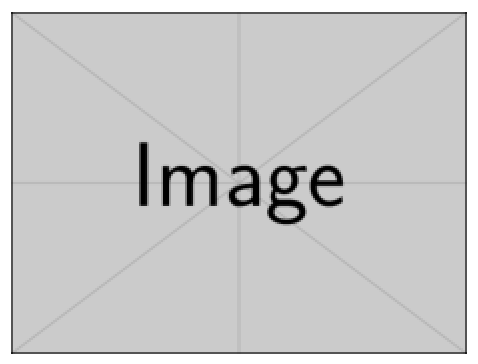
\includegraphics[scale=0.3]{images/fig1}
  \caption{Example of a figure} \label{fig_1}
\end{figure}
As you can see, ``cleverref" allows you to refer to more than just equations: you can refer to \cref{chap_chap2}, or \cref{sec_21}, or \cref{tab_1}, or \cref{fig_1}.
Tables and figures are indexed automatically (see index).

